Data for this project was collected by the US. Army Corps of Engineers Engineer Research and Development Center (ERDC) during October 2015 at the Field Research Facility (FRF) in Duck, NC in the Outerbanks.\footnote{The data can be accessed online at http://chlthredds.erdc.dren.mil/thredds/catalog/frf/projects/bathyduck/catalog.html} The data comes from the Bathyduck project conducted by the Coastal and Hydraulic Laboratory (CHL). We make use of information about wave height, wave number, wave period, and bathymetry. These fields combine information collected by the Argus Beach Monitoring System, the Lighter Amphibious Resupply Cargo (LARC-5) vessel, the Coastal Research Amphibious Buggy (CRAB). 

\begin{figure}[h]
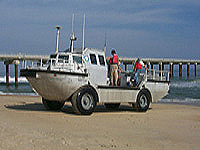
\includegraphics[width=.48\linewidth]{img/LARC.jpg}\hfill
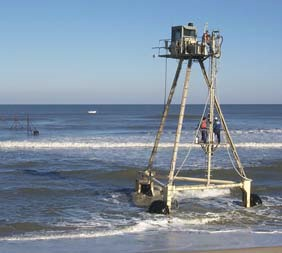
\includegraphics[width=.48\linewidth]{img/CRAB2.jpg}
\caption{The LARC (left) and CRAB (right) instruments are used to measure near coastal bathymetry. Image source: http://www.frf.usace.army.mil/aboutUS/equipment.shtml}
\end{figure}

The following sections discuss in more detail the observations and how they were used. Note the x coordinate of the observations was reversed to correspond to the modeling effort. In physical space, the boundary point used for the 1D problem is located 1150 m from the shoreline. The observations are transformed so that $\textit{x}$ = 0m corresponds to the offshore boundary point and $\textit{x}$ = 1150 m is the shoreline. 

